\documentclass[11pt]{amsart}
%%% WARNING: Do NOT change the page size, fonts, or margins!  Penalties will apply.

\usepackage{placeins} %enables \FloatBarrier, that prevents floats from going below it.
\usepackage{amsmath, amssymb, amsfonts, amsthm, mathtools, bm}
\usepackage{color,comment}
\usepackage{geometry}
\usepackage{hyperref}
\usepackage[english]{babel}
\usepackage{graphicx}
% \usepackage{biblatex}
% \addbibresource{bibliography.bib}

\title{Blending SIR and Predator-Prey Models to Predict the Labor Market}

\author{Jason Vasquez \and Dylan Skinner \and Benjamin Mcmullin \and Ethan Crawford}

\date{December 5 2023}

\begin{document}

\begin{abstract}

    The labor market, including the unemployment rate and the amount of workers looking for jobs, can have a large impact on the economny.
    The more people employed means more money being spent, which in turn means more money being made. 
    Furthermore, rise in unemployment can lead to a recession. Being able to predict the labor market can help us prepare for a recession and help us understand the economy better.
    In this paper, we adapt an SIR model to model the amount of employed, unemployed, and retired individuals.
    Furthermore, we use a quasi predator-prey model to illustrate the oscillation of the two industries commonly known as white-collar and blue-collar.
    
\end{abstract}

\maketitle

We give permission for this work to be shared by ACME Volume 4 instructors and anybody else who may have reasonable motivation.

\section{Background/Motivation}

One thing that is certain in life is that people will always need jobs. Not only this, but people 
will often lose their jobs. Not only this, but people will (eventually) retire from their jobs.
The focus of our project is modeling this situation.

Our investigation navigates the intricate dynamics of employment trajectories and occupational sectors. 
Employing the SIR (Susceptible-Infectious-Recovered) model, typically used for disease dynamics but adapted 
here to study employment dynamics, we aim to comprehend the propagation of employment statuses—specifically, 
the transitions between being employed, unemployed, and retired. A discernible trend has emerged in recent times, 
notably influenced by the technological revolution. The surge in interest and demand for tech-oriented careers 
has prompted a significant shift away from traditional blue-collar professions. This migration has led to a 
dual challenge: a scarcity of skilled workers in the blue-collar sector and an oversaturation of the tech 
industry. Our study extends beyond the conventional SIR model, incorporating elements of a quasi-predator-prey 
framework inspired by ecological models. This approach allows us to capture the nuanced relationship between 
the blue-collar and white-collar industries, offering insights into the cyclical dynamics between these sectors. 
Motivated by the imperative to comprehend and address the consequences of this evolving employment landscape, 
our research aims to contribute valuable insights for informing strategic policies and industry interventions.

\section{Modeling}

\subsection{Theoretical Framework}

The Susceptible-Infectious-Recovered (SIR) model, developed by Kermack and McKendrick in 1927, 
is a foundational mathematical framework for understanding the spread of infectious diseases in populations. 
It divides individuals into susceptible, infectious, and recovered compartments, capturing the dynamics of disease transmission.
In our model, we adapt the SIR model to represent the dynamics of the employment market through the labor force,
unemployed, and retired populations.

\subsection{Previous Work}

We begin by building off the work of ElFadily et. al.~\cite{ElFadily}. In their work, ElFadily et. al. proposed a model
 representing the labor force and unemployed populations. They begin by defining their equations as

\begin{align}
    \begin{split}
        \frac{dL}{dt} &= \gamma U - (\sigma + \mu)L, \\
        \frac{dU}{dt} &= \rho \left(1 - \frac{L_{\tau} + U_{\tau}}{N_c} \right)L_{\tau} + \sigma L - (\gamma + \mu)U, \\
    \end{split}
\end{align}

where $L$ is the labor force, $U$ is the unemployed population, with initial conditions for (1) defined as:

\begin{align}
    \begin{split}
        L&(0) > 0, \quad U(0) > 0, \\
        (L(\theta),U(\theta)) &= (\varphi_1(\theta), \varphi_2(\theta)), \quad \theta \in [-\tau,0], \\
    \end{split}
\end{align}
where $\varphi_i\in C([-\tau, 0], \mathbb{R}^+),\;\; i=1,2$.

The parameters are defined as follows:

\begin{itemize}
    \item $\gamma$: employment rate
    \item $\sigma$: rate of job loss 
    \item $\mu$: mortality rate
    \item $\rho$: maximum population growth rate 
    \item $N_c$: population carrying capacity 
    \item $\tau$: time lag needed to contribute in the reproductive process of a new individual looking for a job
\end{itemize}

\subsection{Modifications: The Retirement Group}
 

With this information in mind, we can begin to adapt this model to fit our needs. We begin by adding a third population, the retired population, $R$.
We can then define our new equations as

\begin{align}
    \begin{split}
        \frac{dL}{dt} &= \gamma U - (\sigma + \mu)L {\color{red}\;- \left(\frac{\Sigma}{L + U}\right) L + \omega\left(\frac{\Sigma}{L + U}\right) R},\\
        \frac{dU}{dt} &= \rho\left(1 - \frac{L + U}{N_c} \right)L + \sigma L -(\mu + \gamma)U,  \\
        \frac{dR}{dt} &= {\color{red}\left(\frac{\Sigma}{L + U}\right) L - \omega\left(\frac{\Sigma}{L + U}\right) R \; - \, \mu R},
    \end{split}
\end{align}

which simplify to 

\begin{align}
    \begin{split}
        \frac{dL}{dt} &= \gamma U - (\sigma + \mu)L {\color{red}\; + \;(\omega R - L)\left(\frac{\Sigma}{L + U}\right)},\\
        \frac{dU}{dt} &= \rho\left(1 - \frac{L + U}{N_c} \right)L_{\tau} + \sigma L -(\mu + \gamma)U  \\
        \frac{dR}{dt} &= {\color{red}(L - \omega R)\left(\frac{\Sigma}{L + U}\right) \; - \, \mu R}.
    \end{split}
\end{align}

One of the first things to note from our equations is the removal of the time lag $\tau$. 
This is because, instead of factoring in people when they are born, we are instead factoring them
in when they turn of working age (16). This reduces unnecessary complexity in our model. Another thing to note
is that we have added two new parameters, $\omega$ and $\Sigma$. We define $\Sigma$ to be the number of people who
retire each year in the United States, and $\omega$ to be the rate at which retired people enter back
into the full-time workforce. We can then define our new initial conditions as:

\begin{align}
    \begin{split}
        L(0) > 0, \quad &U(0) > 0, \quad R(0) > 0, \\
        (L(\theta),U(\theta), R(\theta)) &= (\varphi_1(\theta), \varphi_2(\theta), \varphi_3(\theta)), \quad \theta \in [-\tau,0],
    \end{split}
\end{align}
where $\varphi_i\in C([-\tau, 0], \mathbb{R}^+),\;\; i=1,2,3$. Incorporating nuanced dynamics into our model, we introduce the following terms and elucidate their significance within the equations:

\begin{itemize}
    \item $\pm\left(\frac{\Sigma}{L + U}\right) L$: This term captures the dynamic interplay of individuals retiring from the workforce each time step. By leveraging $\Sigma$, the annual number of retirees, and $L + U$, the total workforce population, we calculate the percentage of individuals retiring at each time step. Multiplying this by $L$, the number of individuals actively engaged in the workforce, yields the precise count of those retiring, excluding unemployed individuals due to their non-participation in this realistic scenario.

    \item $\pm \omega\left(\frac{\Sigma}{L + U}\right) R$: This term accounts for individuals retiring and subsequently re-entering the workforce. The parameter $\omega$ denotes the rate at which retired individuals seamlessly transition back to full-time work. By multiplying $\omega R$—the expected number of retired individuals returning to the workforce—by $\frac{\Sigma}{L + U}$, we ascertain the percentage of recent retirees contributing to the workforce each time step.

    \item $-\mu R$: This term represents the natural attrition of retired individuals through mortality each time step. Its presence acknowledges the inevitable and inherent departure of individuals from the system due to mortality, contributing to a comprehensive understanding of the model's temporal evolution.
\end{itemize}

\subsection{Modifications: The White-Collar and Blue-Collar Groups}

We can further model the labor market by examining the relationship between two industries, commonly referred to as the white-collar and blue-collar industries (ADD CITATION).
In recent years, we have seen an explosion of jobs and interest in the white-collar field, specifically in the tech industry, while the blue-collar industry has seen a decline in interest.
This has led to an oversaturation of the white-collar industry and a scarcity of skilled workers in the blue-collar industry, which in turn has slowed growth in the white-collar industry and led to increased growth in the blue-collar industry.
This cyclical relationship mirrors that of a predator-prey relationship, and we can model it as such.

The classical predator-prey model is given by the following equations: (CITE ME PLEASE)

\begin{align}
    \begin{split}
        \frac{dx}{dt} &= \rho x - a x y, \\
        \frac{dy}{dt} &= -\mu y + \epsilon a x y,
    \end{split}
\end{align}


\section{Results}

We now give the specific values for hyperparameters for our model and how we came to those values. We define the following:

\begin{itemize}
    \item $\sigma = 0.013905$: We derived this value by analyzing comprehensive data on total layoffs and discharges in the United States from 2000 to 2023, as documented by the Federal Reserve Economic Data (FRED) \cite{FRED}. The calculated average resulted in $\sigma = 0.013905$.
    \item $\rho = 0.014577$: The maximum growth rate, denoted as $\rho$, was determined by examining an Excel spreadsheet provided by MacroTrends \cite{MacroTrends}. After averaging the growth rates from 2000 to 2022, we incorporated three standard deviations to arrive at $\rho = 0.014577$.
    \item $\gamma = 0.6062$: The average employment rate from 2000 to 2022, obtained from the Bureau of Labor Statistics \cite{BLS}, led to the computation of $\gamma = 0.6062$.
    \item $\mu = 0.008498$: Derived from an analysis of mortality data from 2000 to 2022 \cite{usafacts}, the mortality rate was calculated by taking the average number of deaths per 100,000 people. This resulted in $\mu = 0.008498$.
    \item $N_c = 260,000,000$: The population of individuals aged 18 and above in the United States in 2022 was calculated to be $260,000,000$, as reported by Kids Count \cite{kidscount}.
    \item $\Sigma = 775,045$: The annual number of retirees in the United States, determined by examining Social Security Administration data from 2000 to 2021 \cite{ssa}, was calculated using the formula:
    \[
        \Sigma = \frac{1}{2021 - 2001}\sum_{i=2001}^{2021}(x_i - x_{i-1})
    \]
    where $x_i$ is the number of retirees in year $i$. This resulted in $\Sigma = 775,045$.
    \item $\omega = 0.063$: The rate at which retired individuals re-enter the full-time workforce, denoted as $\omega$, was identified as 6.3\% or $0.063$ based on research by Maestas \cite{maestas}, resulting in $\omega = 0.063$.
\end{itemize}
We began testing our model by running it for 60 years with differing initial conditions (see figure~\ref{fig:results_lur_1}). We began by using the current numbers for the United States. As you can see,
the model very quickly reaches an equilibrium. Additionally, we can see the total population grow as time goes on, reflecting the expected population growth of the United States.

\begin{figure}[h]
    \centering
    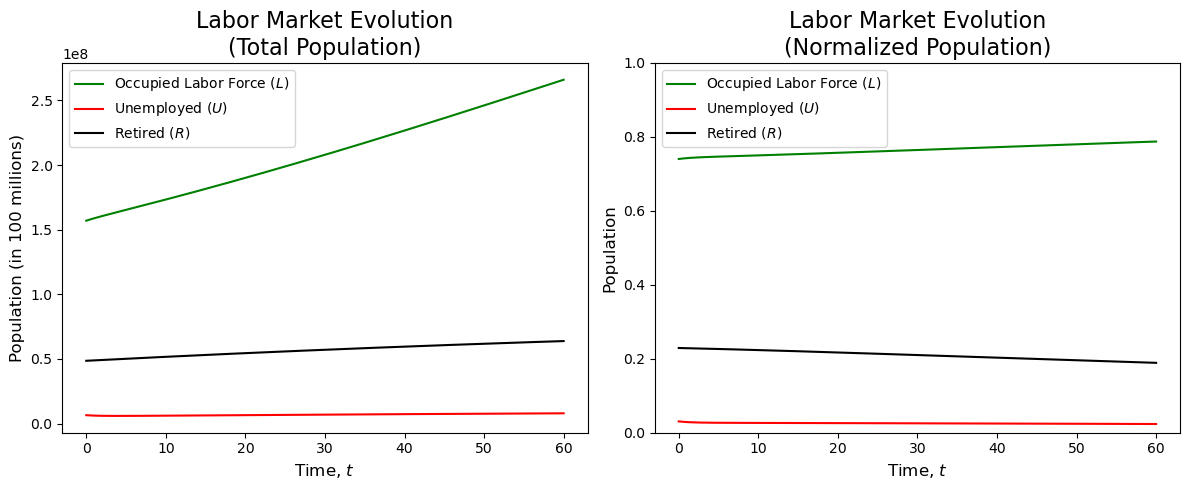
\includegraphics[width=\textwidth]{figures/results_lur_1.png}
    \caption{Initial conditions: $L(0) = 157,000,000$, $U(0) = 6,500,000$, $R(0) = 48,590,000$. These
             numbers reflect the current numbers for the United States. As you can see, the model very quickly
             reaches an equilibrium. Additionally, we can see the total population grow as time goes on, reflecting
             the expected population growth of the United States.}
    \label{fig:results_lur_1}
\end{figure}

To test the robustness of our model, we ran it with different initial conditions. We decreased the number in the labor force, increased the number of 
unemployed, and decreased the number of retired. We then ran the model for 60 years (see figure~\ref{fig:results_lur_2}).

\begin{figure}[h]
    \centering
    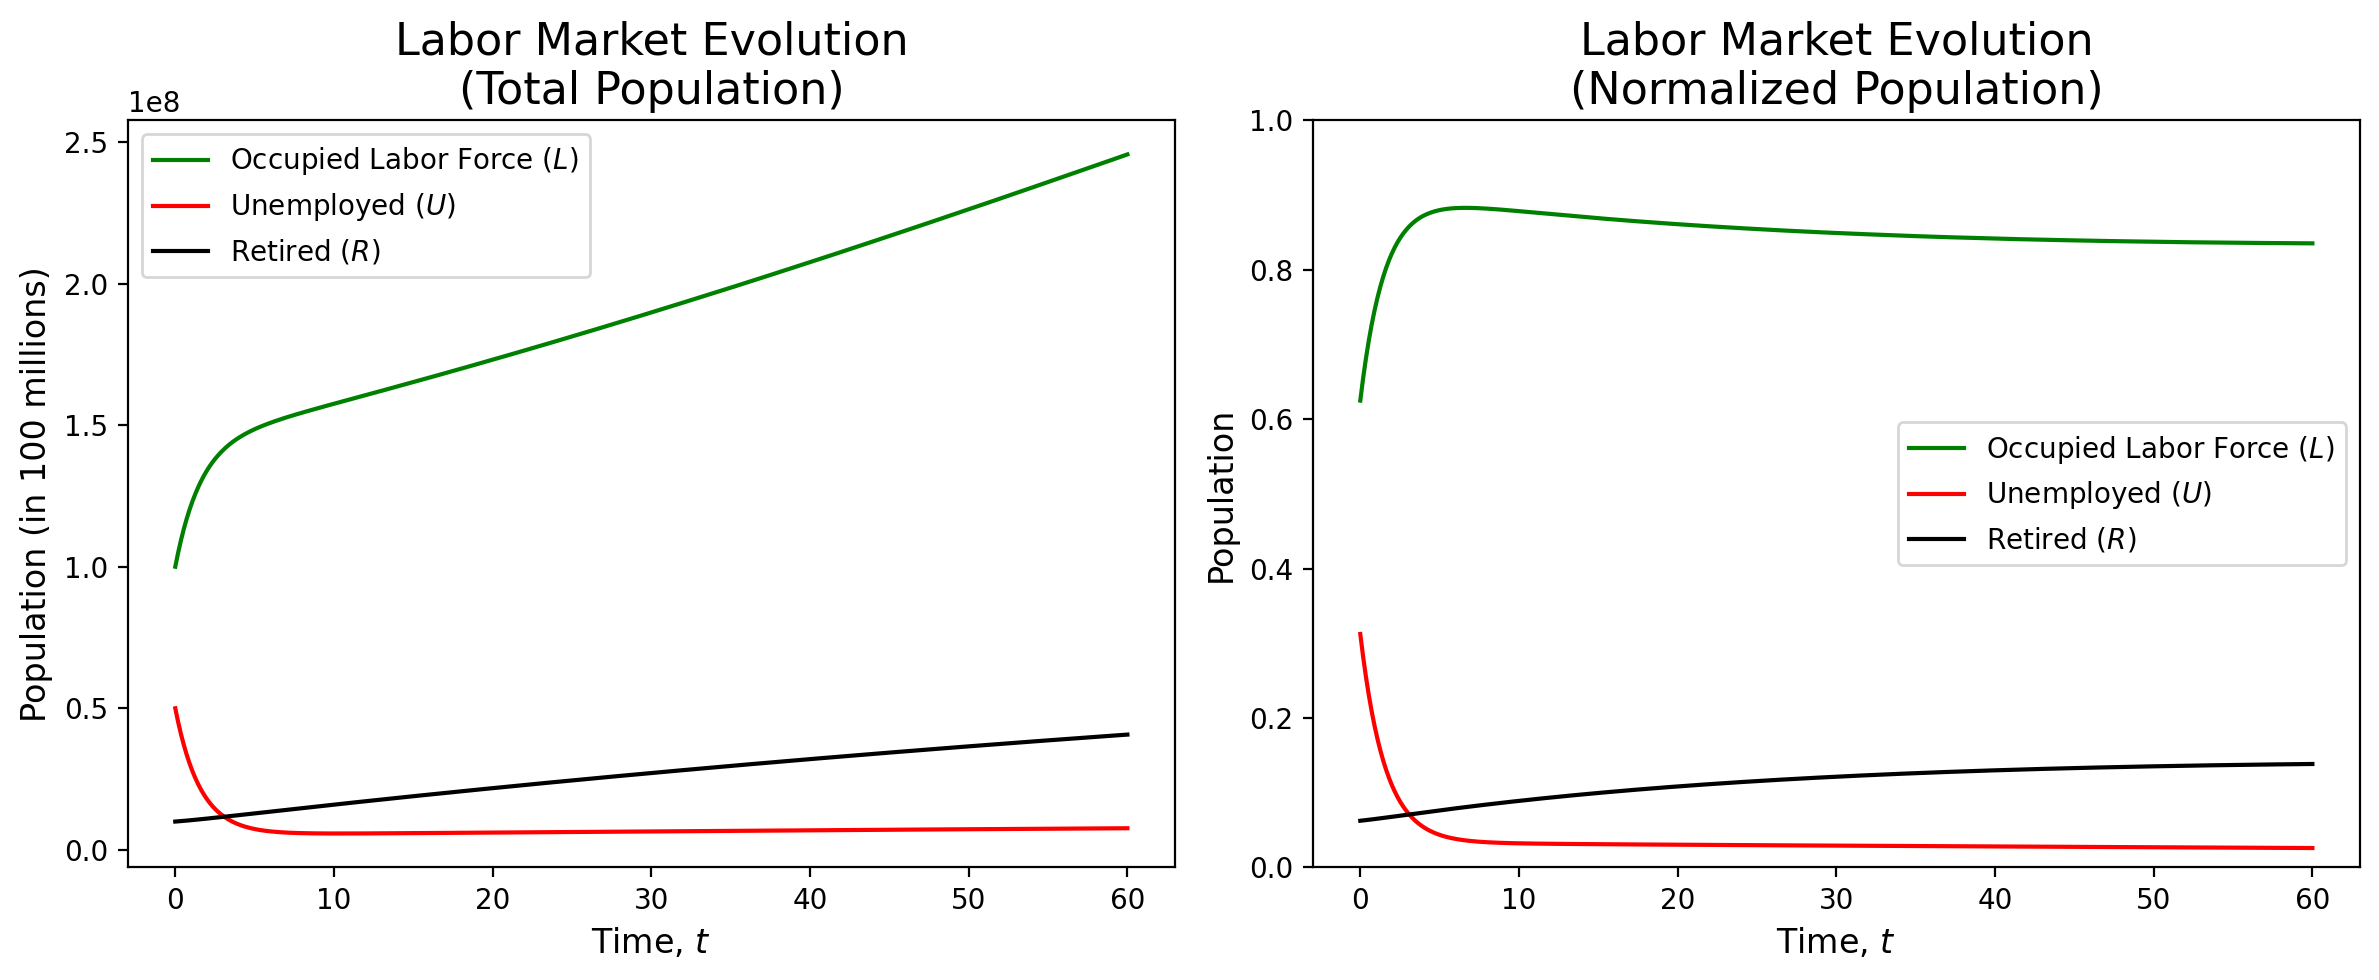
\includegraphics[width=\textwidth]{figures/results_lur_2.png}
    \caption{Initial conditions: $L(0) = 100,000,000$, $U(0) = 50,000,000$, $R(0) = 10,000,000$. As you can see, the model still reaches an equilibrium.}
    \label{fig:results_lur_2}
\end{figure}

\newpage


We ran our model, once again, against a different set of initial conditions. This time, we significantly decreased the number of people in the occupied
labor force, significantly increased the number of unemployed, and moderately decreased the number of retired. We then ran the model for 60 years (see figure~\ref{fig:results_lur_3}).

\begin{figure}[h]
    \centering
    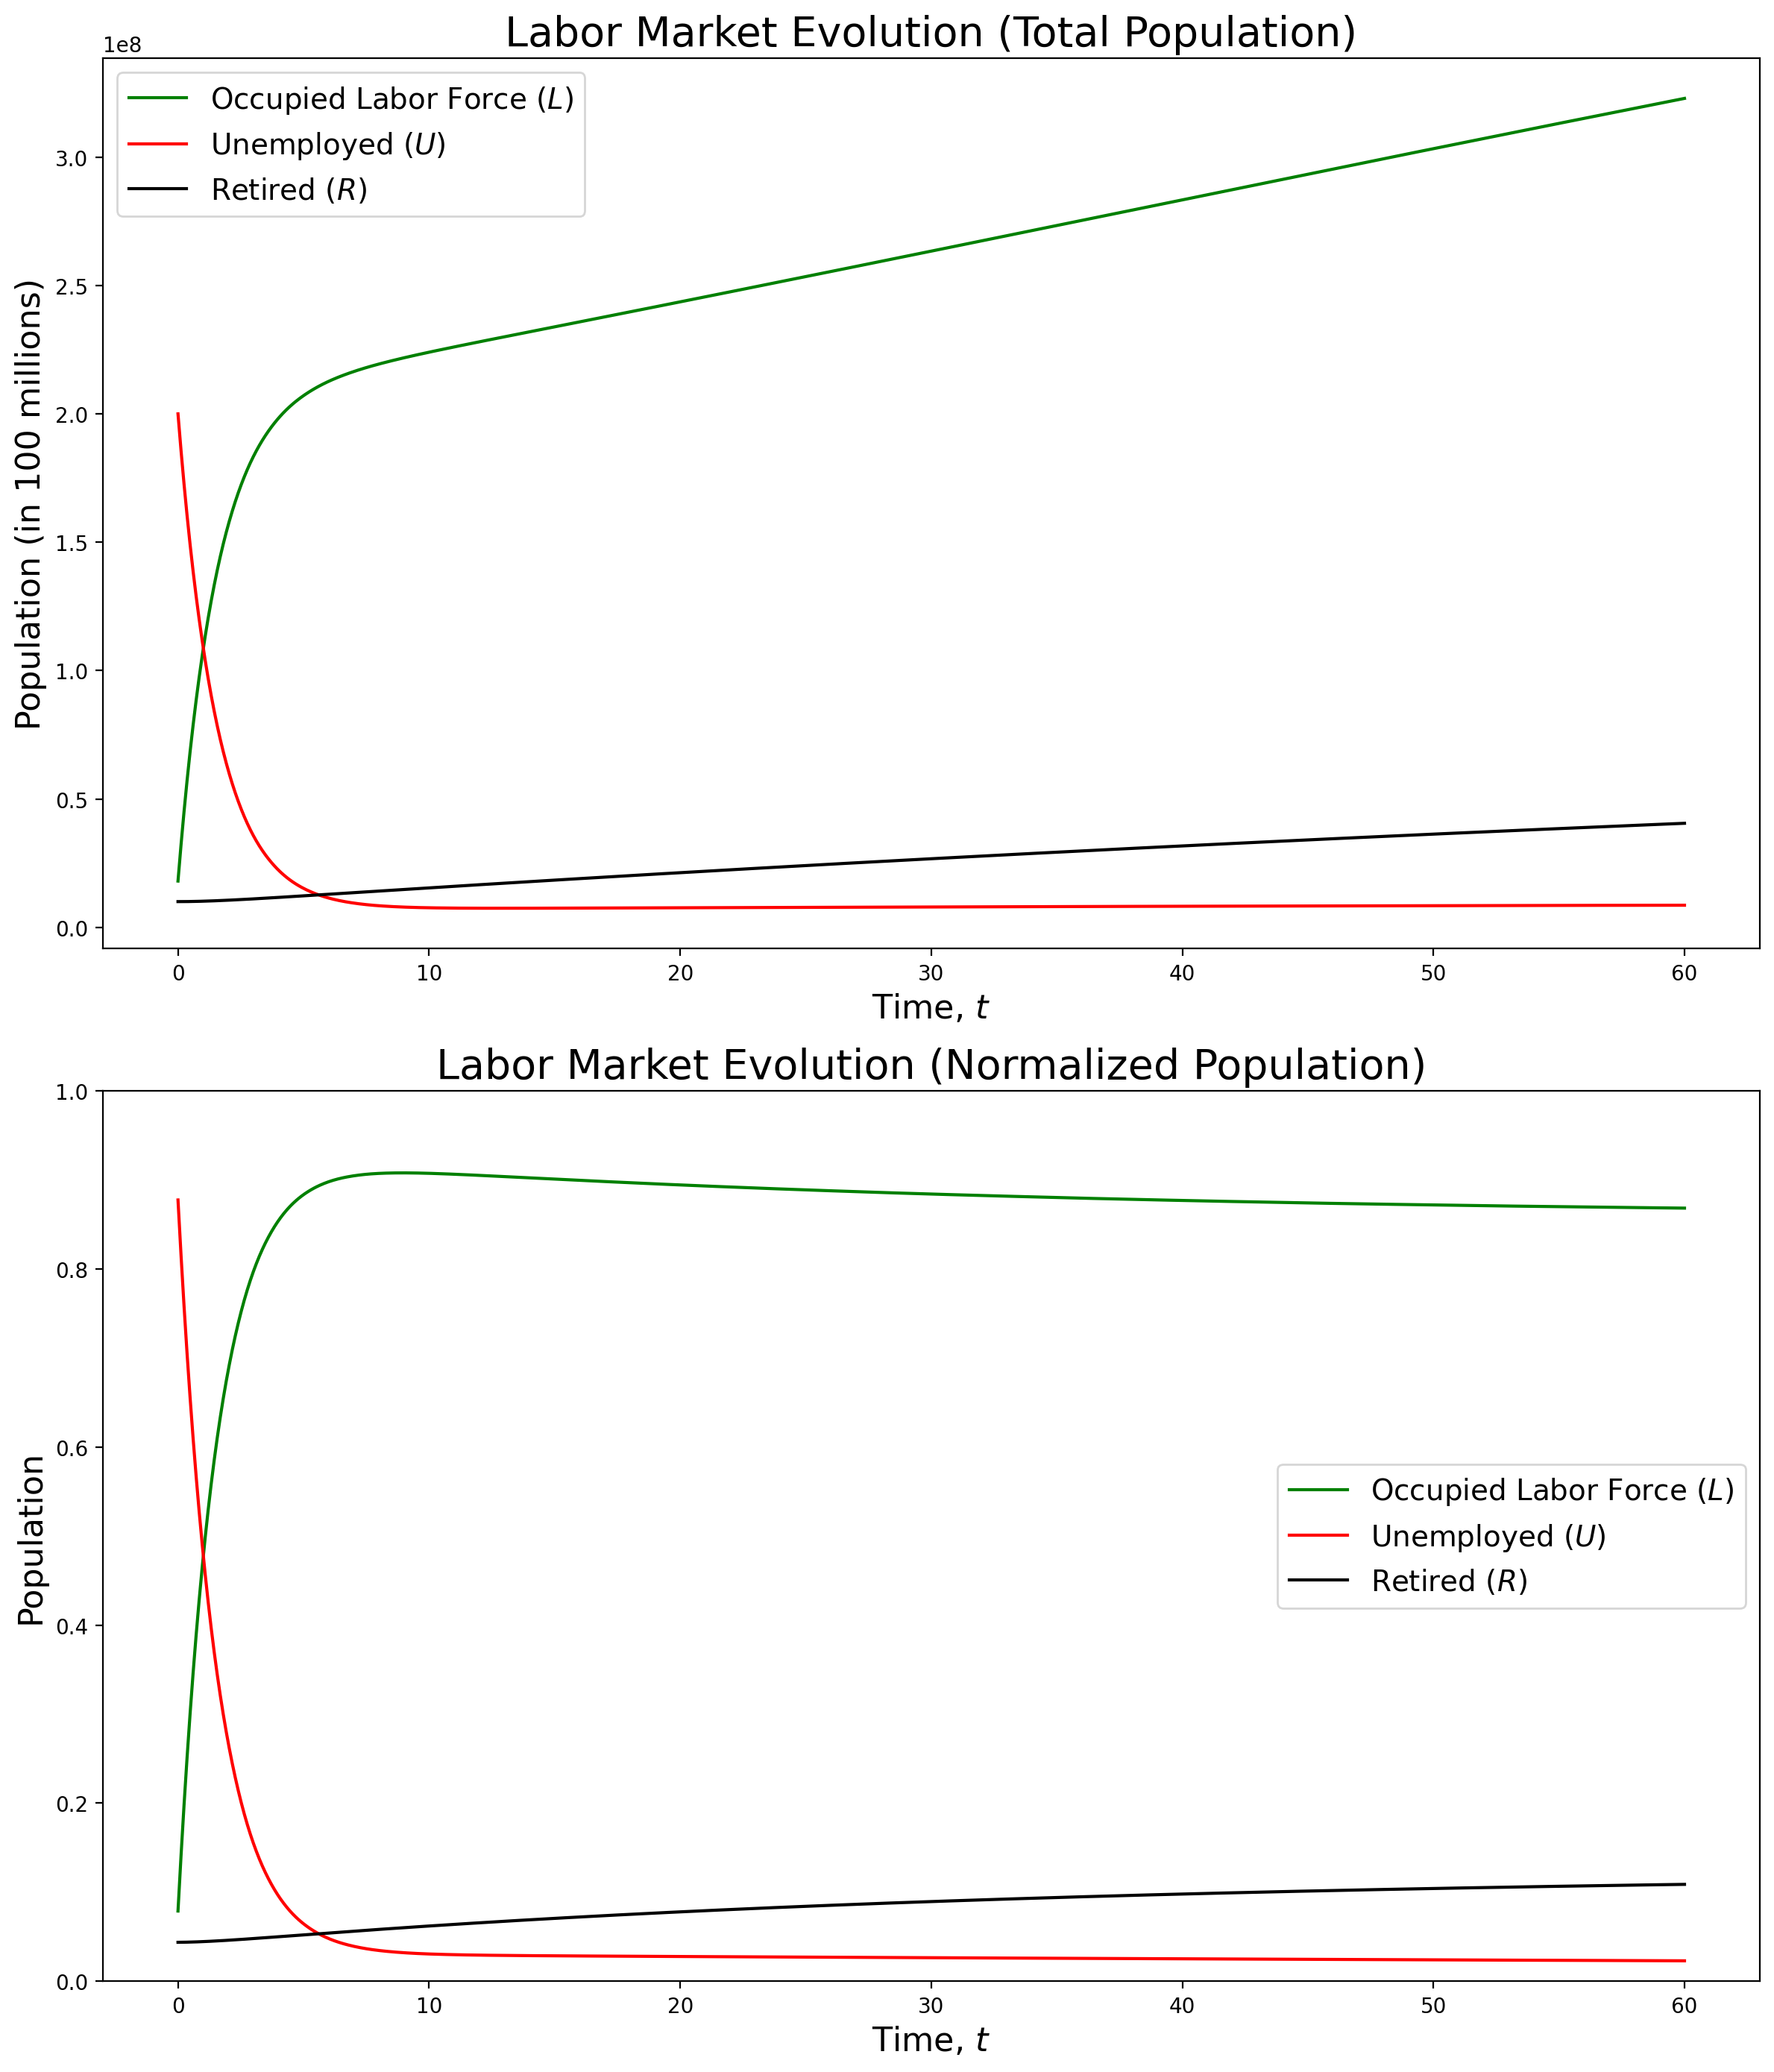
\includegraphics[width=\textwidth]{figures/results_lur_3.png}
    \caption{Initial conditions: $L(0) = 18,000,000$, $U(0) = 200,000,000$, $R(0) = 10,000,000$. As you can see, the model still reaches an equilibrium.}
    \label{fig:results_lur_3}
\end{figure}



\section{Analysis/Conclusions}

Overall, our model of the labor market shows remarkable stability. 
We can see that, regardless of the initial conditions, the model reaches an equilibrium, 
with the number of employed, unemployed, and retired individuals remaining relatively constant.
When we used initial conditions that reflected the current numbers for the United States,
the model saw relatively little change as time went on (see figure~\ref{fig:results_lur_1}).
With initial conditions that represented a larger than average unemployed population, the model corrected itself and reached a
similar equilibrium as the previous model (see figure~\ref{fig:results_lur_2}).
Finally, when presented with initial populations that were flipped, the model still stabilized to the same equilibrium
(see figure~\ref{fig:results_lur_3}).

While harder to see with the scale on the graph, the retired population does increase over time. 
This is because, as the population grows, more people retire and we see a slow but steady growth, as expected.


% Rest of your document goes here

\newpage 
\bibliographystyle{plain}
\bibliography{bibliography}


\end{document}
